\documentclass{robinminion}


\usepackage{amsthm}
\usepackage{enumitem}
\usepackage[round]{natbib}
\usepackage{mllequiv,willemtools}

\graphicspath{{../notes/}}

\makeTheoremDefs


\author{Willem Heijltjes and Robin Houston}
\title{The proof equivalence problem for multiplicative linear logic is \textsc{pspace}-complete v0.3}


\begin{document}

\maketitle

\begin{abstract}
MLL proof equivalence is the problem of deciding whether two proofs in multiplicative linear logic are related by a series of rule permutations.
%
Previous work has shown the problem to be equivalent to a rewiring problem on proof nets, which are not canonical for full MLL due to the presence of the two units.
%
Drawing from recent work on reconfiguration problems, in this paper it is shown that MLL proof equivalence is PSPACE-complete, using a reduction from Nondeterministic Constraint Logic.
\end{abstract}


%\include{s_intro}



\section{MLL}



\begin{figure}
\[
\begin{array}{llll}
	\MLLrule b
 &	\MLLrule 1
 &	\MLLrule p
 &	\MLLrule t
\end{array}
\]
\caption{Inference rules for unit-only \MLL}
\label{fig:MLL}
\end{figure}



\begin{figure}
\[
	\vc{\MLLperm{bb1}} \perm \vc{\MLLperm{bb2}}
\qquad
	\vc{\MLLperm{bp1}} \perm \vc{\MLLperm{bp2}}
\]
\[
	\vc{\MLLperm{bt1}} \perm \vc{\MLLperm{bt2}} \perm \vc{\MLLperm{bt3}}
\]
\[
	\vc{\MLLperm{pp1}} \perm \vc{\MLLperm{pp2}}
\]
\[
	\vc{\MLLperm{pt1}} \perm \vc{\MLLperm{pt2}}
\]
\[
	\vc{\MLLperm{tt1}} \perm \vc{\MLLperm{tt2}}
\]
\caption{Permutations}
\label{fig:permutations}
\end{figure}



The formulae of unit-only multiplicative linear logic are given by the following grammar.
%
\[
	A,B,C \coloneq \bot \mid 1 \mid A\parr B \mid A\tn B
\]
%
The connectives $\tn$ and $\parr$ will be considered up to associativity, and \emph{duality} $\dual A$ is via DeMorgan.
%
A \emph{sequent} $\Gamma,\Delta$ will be a multiset of formulae.
%
Within a sequent, connectives and units will be \emph{named} with distinct elements from an arbitrary set of names $N$, e.g.\
$\named a1\named b\parr\named c1,\named d\bot\named e\tn\named f\bot$.
%
This allows to 1) avoid using the notion of \emph{occurrence}, and instead refer to subformulae by the name of their root connective, as e.g.\ $\named bA$, 2) distinguish the two proofs of the above sequent while using standard multiset sequents, and 3) easily extract proof nets, as graphs using the names of connectives as vertices.
%
Names will mostly be left implicit.



Proofs are constructed from the inference rules in Figure~\ref{fig:MLL}.
%
The names of connectives are preserved through inferences.
%
Only cut-free proofs are considered, and no cut-rule is added.
%
\emph{Permutations} of inference rules are displayed in Figure~\ref{fig:permutations}; the symmetric variants of the last two permutations, \emph{par-tensor} and \emph{tensor-tensor}, have been omitted.



\begin{definition}
\label{def:equivalence}
%
\emph{Equivalence} of proofs in (cut-free, unit-only) multiplicative linear logic $(\perm)$ is the congruence generated by the permutations given in Figure~\ref{fig:permutations}.
%
\emph{\MLL\ proof equivalence} is the problem of deciding whether two given proofs are equivalent.
%
\end{definition}



The motivation to consider proofs up to equivalence is three-fold.
%
Firstly, there is the strong intuition that the order of permutable inferences does not contribute to the essential content of the proof.
%
Secondly, a technical motivation is that cut-elimination in \MLL\ incorporates permutation steps, and composition via cut-elimination is only associative up to permutations.
%
Thirdly, equivalent proofs are identified in natural models of multiplicative linear logic such as coherence spaces, and in the categorical semantics of \MLL, $\star$-autonomous categories.



In one of several possible definitions, a \emph{$\star$-autonomous category} \citep{Barr-1979} is a symmetric monoidal category $(\mathcal C,\tn,1)$ with:
%
\begin{itemize}
	
	\item
	a \emph{duality}, a contravariant functor $\dual-$ such that $A\cong\dual*A$, and

	\item
	\emph{closure}, an adjunction $-\tn B \dashv \dual{(B\tn\dual-)}$ for any object $B$,

\end{itemize}
%
satisfying natural coherence conditions.
%
%The category $\textsc{mll}(\emptyset)$ of unit-only \MLL-formulae and equivalence classes of proofs is a $\star$-autonomous category.
%
The category with as objects unit-only \MLL-formulae and as morphisms $A\to B$ the equivalence classes of proofs of $\dual A\parr B$, denoted $\textsc{mll}(\emptyset)$, is a $\star$-autonomous category.
%
The present formulation of formulae induces two forms of \emph{strictness}, instances where isomorphisms of the definition are identities: DeMorgan duality means $A=\dual*A$, while
%, one-sided sequents mean the closure adjunction is an equivalence of categories, 
associativity is an identity by decree.
%
Modulo strictness, $\textsc{mll}(\emptyset)$ is the \emph{free} $\star$-autonomous category over the empty category $\emptyset$.
%
This means that \emph{any} $\star$-autonomous category is a model of the logic, and that \MLL\ proof equivalence is the \emph{word problem} for $\star$-autonomous categories, the problem of deciding when two representations of morphisms denote the same morphism.




%The \emph{free $\star$-autonomous completion} $\star$-\textsc a$(\mathcal C)$ of a category $\mathcal C$ is characterised by a functor $i\colon\mathcal C\to\star$-\textsc a$(\mathcal C)$ such that any functor $\mathcal C\to \mathcal D$ into a $\star$-autonomous cateogry $\D$ factors uniquely (up to canonical isomorphism) as the composition of $i$ with a functor $\star$-\textsc a$(\mathcal C)\to\D$ preserving $\star$-autonomous structure.
%%
%\[
%\begin{tikzpicture}[auto]
%	\node (C) at (0,0) {$\mathcal C$};
%	\node (*AC) at (2,0) {$\star$-\textsc a$(\mathcal C)$};
%	\node (D) at (1,1) {$\mathcal D$};
%	\draw [->] (C) -- node {$i$} (*AC);
%	\draw [->] (C) -- (D);
%	\draw [->,dashed] (*AC) -- node {$!$} (D);
%\end{tikzpicture}
%\]
%%



\subsection{Proof nets}

A partial solution to the \MLL\ proof equivalence problem is provided by proof nets.


\begin{definition}
\label{def:proof nets}
%
For a sequent $\Gamma$,
\begin{itemize}

	\item
	a \emph{linking} $\links$ is a function from the names of $\bot$-subformulae to the names of $1$-subformulae,

	\item
	a \emph{switching graph} for $\links$ is an undirected graph over the names of $\Gamma$, with for every subformula $\named aA\named c\tn\named bB$ the edges $a-c$ and $b-c$, for every subformula $\named aA\named c\parr\named bB$ either the edge $a-c$ or the edge $b-c$, and for every subformula $\named a\bot$ the edge $a-\links(a)$,

 	\item
	a \emph{proof net} $\links$ or $(\Gamma,\links)$ is a linking $\links$ such that every switching graph is acyclic and connected.

\end{itemize}
\end{definition}


\noindent
An edge $a-\links(a)$ in a proof net or switching graph is a \emph{link} or \emph{jump}.



\begin{definition}
\label{def:proof net equivalence}
%
A \emph{permutation} between proof nets is the redirection of exactly one link.
%
\emph{Equivalence} $(\perm)$ of proof nets over a sequent $\Gamma$ is the congruence generated by permutations.
%
\end{definition}


\noindent
There is no canonical interpretation of a proof as a proof net, since the introduction rule for $\bot$ in proofs joins a $\bot$-formula to a sequent, rather than a formula.



\begin{definition}
\label{def:proofs to nets}
%
The relation $(\toNet)$ interprets a proof $\Pi$ for a sequent $\Gamma$ by a linking $\links$ as follows:
% 
$\Pi\toNet\links$ if for each $\named a\bot$ in $\Gamma$, if $\Delta$ is the context of the inference introducing $\named a\bot$, as illustrated below, then $\links(a)$ is the name of some $1$ in $\Delta$.
\[
	\infer[\MLLlabel b]{\Delta,\named a\bot}{\Delta}
\]
%
\end{definition}



\begin{proposition}[\citeauthor{DR89}, \citeyear{DR89}]
\label{prop:correctness and sequentialisation}
%
For a proof $\Pi$ with conclusion $\Gamma$, if $\Pi\toNet\links$ then $\links$ is a proof net for $\Gamma$.
%
For a net $\links$ for $\Gamma$, there is a proof $\Pi$ of $\Gamma$ such that $\Pi\toNet\links$ (\emph{sequentialisation}).
%
\end{proposition}


\noindent
Proof nets are canonical representations of proofs in the absence of units: they factor out the permutations among tensor- and par-inferences, which are the last three permutations in Figure~\ref{fig:permutations}.
%
Equivalence of proof nets is generated by the remaining equations, the permutations on $\bot$-introduction.



\begin{proposition}[\citeauthor{HughesMLLProofNets}, \citeyear{HughesMLLProofNets}]
\label{prop:proof nets work}
%
For proofs $\Pi$, $\Pi'$ and proof nets $\links$, $\links'$ such that $\Pi\toNet\links$ and $\Pi'\toNet\links'$, $\Pi\perm\Pi'$ if and only if $\links\perm\links'$.
%
\end{proposition}


\noindent
\MLL\ proof equivalence is the problem of deciding equivalence of proof nets.


\subsection{Notation}


We will use a concise diagrammatic notation for sequents and proof nets.
%
The units $1$ and $\bot$ are represented by a circle $\circ$ and a disc $\bullet$ respectively.
%
A tensor is represented by a line connecting both subformulae, and a par by juxtaposition: if $A$ and $B$ are represented by \raisebox{-0.3\height}{
\includegraphics[scale=0.75]{hex-A.pdf}}
and \raisebox{-0.3\height}{
\includegraphics[scale=0.75]{hex-B.pdf}},
%
then $A\parr B$ is \raisebox{-0.3\height}{
\includegraphics[scale=0.75]{hex-AparB.pdf}}
and $A\tn B$ is \raisebox{-0.3\height}{
\includegraphics[scale=0.75]{hex-AtnB.pdf}}.
%
A tensor of multiple elements is denoted by stringing them together in a line, so $A\tn B\tn C$ is
\raisebox{-0.3\height}{
\includegraphics[scale=0.75]{hex-AtnBtnC.pdf}}.
%
Boxes play the role of parentheses around par-formulae, so $(A\parr B)\tn C$ is drawn as \begin{center}{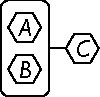
\includegraphics[scale=1]{hex-AparBtnC.pdf}}\end{center}

\noindent For example, this sequent
\[ \vdash \bot\tn\bot, \bot\tn\bot, \bot\tn\bot, \bot\tn\bot, 1, \{[(1\parr 1\parr 1)\tn(1\parr 1\parr 1)]\parr 1\parr (\bot\tn\bot\tn\bot)\parr 1\}\tn\bot \]
could be drawn like this:
\begin{center}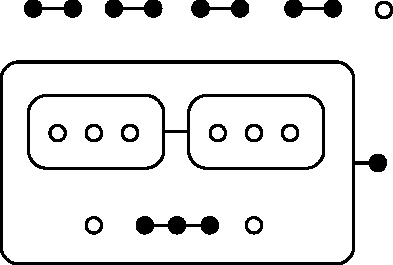
\includegraphics[scale=0.75]{example-sequent.pdf}\end{center}

\noindent We represent a proof net by drawing an arrow from each $\bullet$ to some $\circ$. For example, one proof net on the above sequent is
\begin{center}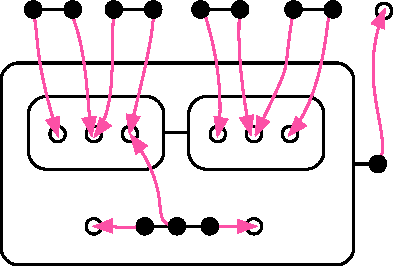
\includegraphics[scale=0.75]{example-sequent-proofnet.pdf}\end{center}











%NOTE: need 'octopus' terminology here

%NOTE: will we need to count arms often enough to make it worthwile to write $|\Gamma|_\bot$ for the number of $\bot$-occurrences in a sequent $\Gamma$?


\section{Equivalence in the absence of $~\protect\parr$}





Let a \emph{1-alternation} sequent be one over formulae of the form $1$ or $\bot\tn\ldots\tn\bot$, where the number of $\bot$-subformulae is at least 2.
%
Such a sequent is inhabited exactly when the number of formulae in the sequent is one greater than the total number of $\bot$-subformulae it contains.
%
An inhabited 1-alternation sequent with only one tensor-formula, i.e.\ a sequent of the form $\1,\ldots,\1,\bot\tn\ldots\tn\bot$ with $n$ $\bot$-subformulae and $n$ $1$-subformulae, will admit $n!$ different proof nets, each with $n$ links.
%
Since no link can re-attach, its equivalence classes are singletons.



\begin{proposition}
\label{prop:level0 max binary}
%
For a 1-alternation sequent with at least two tensor-formulae there are at most two equivalence classes of proof nets.
%
\end{proposition}



\begin{figure}[p]
\[
\begin{array}{ccc}
	\basenet 1213 & \perm & \basenet 3213 \\ \\[-6pt] \vperm && \vperm \\ \\[-6pt]
	\basenet 1223 &		  & \basenet 3212 \\ \\[-6pt] \vperm && \vperm \\ \\[-6pt]
	\basenet 1323 &		  & \basenet 3112 \\ \\[-6pt] \vperm && \vperm \\ \\[-6pt]
	\basenet 1321 &		  & \basenet 3132 \\ \\[-6pt] \vperm && \vperm \\ \\[-6pt]
	\basenet 2321 &		  & \basenet 2132 \\ \\[-6pt] \vperm && \vperm \\ \\[-6pt]
	\basenet 2331 & \perm & \basenet 2131
\end{array}
\qquad
\begin{array}{ccc}
	\basenet 1312 & \perm & \basenet 1332 \\ \\[-6pt] \vperm && \vperm \\ \\[-6pt]
	\basenet 2312 &		  & \basenet 1232 \\ \\[-6pt] \vperm && \vperm \\ \\[-6pt]
	\basenet 2313 &		  & \basenet 1231 \\ \\[-6pt] \vperm && \vperm \\ \\[-6pt]
	\basenet 2113 &		  & \basenet 3231 \\ \\[-6pt] \vperm && \vperm \\ \\[-6pt]
	\basenet 2123 &		  & \basenet 3221 \\ \\[-6pt] \vperm && \vperm \\ \\[-6pt]
	\basenet 3123 & \perm & \basenet 3121
\end{array}
\]
\caption{The two equivalence classes of nets for $\1,\1,\1,\bot\tn\bot,\bot\tn,\bot$}
\label{fig:2x12 nets}
\end{figure}



\begin{proof}
%
It will be shown by induction on the number of $\bot$-formulae in $\Gamma$ that every proof net for $\Gamma$ belongs to one of two equivalence classes.
%
For the base case, the smallest inhabited sequent with two tensor-formulae is the following.
\[
	\1,\1,\1,\bot\tn\bot,\bot\tn,\bot
\]
It has two equivalence classes of 12 proof nets each, displayed in Figure~\ref{fig:2x12 nets}.



For the inductive step, let $\Gamma$ be the following sequent.
\[
	\Delta,A\tn\named a\bot,\named x\1
\]
There are two cases: 1) where $A$ is a tensor-formula, and 2) where $A$ is $\bot$ and where, for the induction hypothesis to apply, $\Delta$ contains at least two tensor-formulae.
%
For both cases, it will be shown that any net $\links$ for $\Gamma$ is equivalent to a net $\links'$ where $\named a\bot$ connects to $\named x1$, and is the only link to do so.
%
This reduces equivalence on $\Gamma$ to equivalence on $\Delta,A$ in case 1, and on $\Delta$ in case 2, so that the induction hypothesis applies.


Let $\named a\bot$ connect to $\named y\1$ in $\Delta$.
%
For case 1, let $A$ be $A'\tn\named c\bot$; for case 2, let $A=\named c\bot$.
%
Then $\links'$ is obtained by adjusting $\links$ as follows.
\begin{itemize}

	\item
Let $\edge cz$, i.e.\ $\named z\1$ is the target of the jump from $\named c\bot$.	
%
Ensure that $\named z\1$ is the only target shared between jumps in $A$ and in $\Delta$, by moving any other such jump from $\Delta$ to $\named z\1$.

	\item
If there are multiple links connecting to $\named x\1$, select one $b-x$ for some $\named b\bot$ in a tensor-formula $B$.
%
Re-attach the others to the target of another jump out of $B$, of which there must be at least one.

	\item
Since $A$ is only connected via $\named z\1$, there is a link $\edge dz$ connecting $B$ to $A$ (though $\named d\bot$ is not necessarily a subformula of $B$).
%
Re-attach $\named d\bot$ to $\named y\1$, then $\named a\bot$ to $\named x\1$, and $\named b\bot$ to $\named z\1$.

\end{itemize}

\end{proof}




\begin{proposition}
\label{prop:level0 may-connect path}
%
In a proof net for a 1-alternation sequent a link $\edge{\named a\bot}{\named b\1}$ can be permuted to $\edge{\named a\bot}{\named c\1}$ if and only if there is a path in the net from $b$ to $c$ not passing through $a$.
%
\end{proposition}


If a link $\edge ab$ may be reconnected as $\edge ac$ it is said that $a$ \emph{may connect to} $c$. 
%
By the above proposition, it is immediate that if $a$ and $b$ may both connect to $c$, then after actually reconnecting $\edge ac$, still $b$ may connect to $c$.



Consider the following naming scheme for the units in a 1-alternation sequent $\Gamma$ with tensor-formulae $A_1,\dotsc,A_n$.
%
\begin{itemize}

	\item
The first $\1$ in $\Gamma$ is named $N$, the remaining ones are named with the numbers $n+1,\dotsc,m$.

	\item
A $\bot$-formula in $A_i$ is named by a pair $(i,k)$, where $k=N$ for the first $\bot$-formula in each $A_i$, and for the remaining $\bot$-formulae in all $A_i$, each $k$ is a distinct number in $n+1,\dotsc,m$.

\end{itemize}
%
The naming scheme suggests a linking for $\Gamma$, where $\edge{(i,k)}{k}$ for each $\bot$-formula; i.e\ the first $\bot$-subformula of each tensor-formula connects to $\named N\1$, while other $\bot$-subformulae connect uniquely to the remaining $\1$-subformulae.



A net for $\Gamma$ is interpreted as a combinatorial permutation (an automorphism on $\{1,\dotsc,m\}$) as follows.
%
\begin{definition}
To a proof net $\links$ for a 1-alternation sequent $\Gamma$ named as above, associate the \emph{permutation} $\prm:\{1,\dotsc,m\}\to\{1,\dotsc,m\}$ given by:
\[
	\prm(k) = 
	\begin{cases}
		i				& \text{ if $(i,k)$ may connect to $N$; otherwise,}
	\\	j				& \text{ where $\edge{(i,k)}j$.}
	\end{cases}
\]
The \emph{parity} of $\links$ is the parity of its permutation.
\end{definition}


To see that $\prm$ is injective, consider the following.
\begin{itemize}
	\item The domains of $i$ and $j$ are $1,\dotsc,n$ and $n+1,\dotsc,m$ respectively, and hence disjoint.
	\item Exactly one $\bot$-formula in each $A_i$ may connect to $N$ because of connectedness and acyclicity, since if a $\bot$-formula may connect to $N$ it has a path to $N$ (Proposition~\ref{prop:level0 may-connect path}).
	\item If two $\bot$-formulae have the same target, which means they are in different tensor-formulae, at least one may connect to $N$ via the other tensor-formula, which must have a path to $N$ by the above.
\end{itemize}



\begin{proposition}
\label{lem:level0 min binary}
Re-attaching a jump in a net $\links$ preserves its parity. 
\end{proposition}


\begin{proof}
Let $\links$ be a net for $\Gamma$, with $\Gamma$ named as above, and let the link $\edge{(i,k)}x$ in $\links$ re-attach as $\edge{(i,k)}y$, forming $\links'$.
%
There are two cases, depending on whether $(i,k)$ may connect to $N$.
%
If so, using Proposition~\ref{prop:level0 may-connect path}, the re-wiring preserves which $\bot$-formulae may connect to $N$, since for any path to $N$ via $\edge{(i,k)}x$ in $\links$ there is a path to $N$ via $\edge{(i,k)}y$.
%
Then the permutation of $\links'$ is that of $\links$.


If $(i,k)$ may not connect to $N$, let the path from $x$ to $y$ run via the following $\bot$- and $\1$-vertices.
\[
	x=x_1, (i_1,j_1), (i_1,k_1), x_2, (i_2,j_2), \dotsc, (i_n,k_n), x_{n+1}=y 	
\]
Note that the $\bot$-formulae $(i_a,j_a)$ may connect to $N$.
%
On the relevant domain, this gives the following permutation for $\links$.
\[
\left(\begin{array}{ccccccc}
	j_1 & \dotso & j_n &  k  & k_1 & \dotso & k_n \\
	i_1 & \dotso & i_n & x_1 & x_2 & \dotso & x_{n+1}
\end{array}\right)
\]
In $\links$, where $(i,k)$ connects to $y$, the $\bot$-formulae $(i_a,k_a)$ may connect to $N$, giving the following permutation.
\[
\left(\begin{array}{ccccccc}
	j_1 & \dotso & j_n &    k    & k_1 & \dotso & k_n \\
	x_1 & \dotso & x_n & x_{n+1} & i_1 & \dotso & i_n
\end{array}\right)
\]
The parity of both permutations is the same if and only if the relative permutation, below, is even.
\[
\left(\begin{array}{ccccccc}
	i_1 & \dotso & i_n & x_1     & x_2 & \dotso & x_{n+1} \\
	x_1 & \dotso & x_n & x_{n+1} & i_1 & \dotso & i_n
\end{array}\right)
\]
This is the case, as it is obtained by the exchange of $x_a$ and $i_a$ for each $a\leq n$, and subsequently the exchange of $x_{n+1}$ and each $i_a$ in turn.

\end{proof}

















\section{Par}



\begin{definition}
A \emph{sub-sequent} $\Delta\leq\Gamma$ of a sequent $\Gamma$ is a sequent consisting of disjoint subformulae of $\Gamma$, preserving names.
\end{definition}


\begin{definition}
A \emph{subnet} $(\Gamma',\links') \leq (\Gamma,\links)$ of a proof net is a net such that $\Gamma'\leq\Gamma$ and $\links'$ is $(\links|_{\Gamma'})$, the restriction of $\links$ to $\Gamma'$.
\end{definition}


The root vertices of $\Gamma'$ are the \emph{ports} of the sub-sequent $\Gamma'$ and of the subnet $(\Gamma',\links')$.
%
A \emph{scope} of a par $\named v\parr$ is a subnet that has $v$ as a port.
%
In a proof net, the \emph{kingdom} and the \emph{empire} of a par are respectively its smallest and largest scope.



The scopes of a par correspond to the possible subproofs of its introduction rule in a sequentialisation of the proof net that it occurs in.
%
In the graph of a proof net, the scope of a par $\named v\parr$ may be \emph{contracted} to a single vertex $v$ by removing all vertices except $v$ and re-attaching all arcs connecting to removed vertices to $v$.
%

[[ ADD ILLUSTRATED EXAMPLE ]]

%
The contraction of scopes may replace the switching condition as a correctness criterion.
%
The following is a variant of the local retraction algorithm by Danos \cite{Danos-1990}.


\begin{proposition}
\label{prop:scoping correctness}
A linking $\links$ for a sequent $\Gamma$ is a proof net if and only if each $\named v\parr$ is a port of a sub-sequent $s(v)\leq\Gamma$ such that:

\begin{enumerate}
	\item
sub-sequents are strictly nested: if $\named w\parr$ occurs in $s(v)$ then $s(w)<s(v)$; and
	\item
for each $\named v\parr$, the graph $\sigma(v)=(s(v),\links|_{s(v)})$ becomes a tree when all immediate sub-sequents $s(w)$ are contracted.
\end{enumerate}

\end{proposition}


\begin{proof}
For the `if' direction, it follows by induction on the nesting of sub-sequents that each graph $\sigma(v)$ satisfies the switching condition.
%
For the `only if' direction, given a sequentialisation of $(\Gamma,\links)$, a sub-sequent $s(v)\leq\Gamma$ for each $\named v\parr$ is found by taking the conclusion $\Delta, A\named v\parr B$ of its introduction rule, below.
\[
	\infer{\Delta,A\named v\parr B}{\Delta,A,B}
\]
\end{proof}





[[ IDEA: the following could help simplify octopus-arithmetic ]]


\begin{definition}
The \emph{balance} of a sequent is the number of $\bot$s minus the number of $\parr$s and comma's.
%
A sequent is \emph{balanced} if its balance is zero.
\end{definition}

An unbalanced sequent is uninhabited: a positive balance guarantees a cycle in any switching graph, for any linking, while a negative balance similarly guarantees disconnectedness.

An early conjecture of Girard, which turned out to be false, was that a sequent is inhabited if and only if it is balanced. [[FIND CITATION (probably TCS87)]]










\section{Proof nets and constraint graphs}



\newcommand\alt{\underline}

[[ NOTE: we should decide on notation for steps versus paths in permutation relations ]]



\begin{definition} 
A \emph{non-deterministic constraint graph} (\textsc{ncg}) $G=(V,E,c,v,w)$ consists of a set $V$ of vertices with \emph{minimum inflow constraint} $c\colon V\to\mathbb N$, and a set $E$ of at most one undirected edge $e$ per vertex-pair $v(e)=\{v_1,v_2\}$, with \emph{weight} $w\colon E\to N$.

A (partial) \emph{configuration} of an \textsc{ncg} is a (partial) function $\gamma\colon E\to V$ such that
\begin{itemize}
	\item
for every edge $e$, $\gamma(e)\in v(e)$ or (in the partial case) $\gamma(e)$ is undefined, and
	\item
for every vertex $v$, the sum of its inflow weights is at least its inflow constraint, $\sum\{w(e)\mid \gamma(e)=v\}\geq c(v)$.
\end{itemize} 

A \emph{reconfiguration step} $\gamma\sim\delta$ connects two (partial) configurations for an \textsc{ncg} $G$ that differ in the assignment of exactly one edge.

\end{definition}


The \emph{(partial) \textsc{ncg}-reconfiguration problem} is the problem of deciding when two (partial) configurations are connected by a path in the graph of (partial) configurations and reconfiguration steps.

\begin{theorem}[\cite{demaine}]
\textsc{ncg}-reconfiguration is \textsc{pspace}-complete.
\end{theorem}

\begin{proposition}
Partial \textsc{ncg}-reconfiguration is \textsc{pspace}-complete.
\end{proposition}

\begin{proof}
There is a path between total configurations $\gamma$ and $\delta$ in partial \textsc{ncg}-reconfiguration if and only if there is one in \textsc{ncg}-reconfiguration, for the following two reasons.
%
Firstly, if $\gamma\sim\delta$ are partial configurations, they may be completed to total configurations $\gamma'\sim\delta'$ or $\gamma'=\delta'$.
%
Secondly, if $\gamma'$ and $\gamma''$ are total configurations that both agree with a partial configuration $\gamma$ where it is defined, then $\gamma'$ and $\gamma''$ are connected in \textsc{ncg}-reconfiguration by re-assigning the values where they disagree.
%
\end{proof}


For a graph $G=(V,E,c,v,w)$ let $|V|$ and $|E|$ denote the number of vertices and edges, respectively, and let $|c|$ and $|w|$ denote the sum of all inflow constraints, $\sum_{v\in V}c(v)$, and the sum of all edge weights, $\sum_{e\in E}w(e)$.


Let $A^n$ denote the sequent of $n$ copies of a formula $A$, and for a sequent $\Gamma=A_1,\dotsc,A_n$ let $\bigotimes\Gamma=A_1\tn\dotso\tn A_n$ and $\bigparr\Gamma=A_1\parr\dotso\parr A_n$.



\begin{definition}
\label{def:graph interpretation}
The \emph{interpretation} $\itn G$ of an \textsc{ncg} $G=(V,E,c,v,w)$ is a sequent constructed as follows.
%
Let $V=\{v_1,\dotsc,v_n\}$ and $E=\{e_1,\dotsc,e_m\}$ where $|V|=n$ and $|E|=m$.

The interpretation of a vertex $v_k$ is the formula
\[
	\itn{v_k} = \bigparr\big(C^{m\times c(v_k)} \big)\parr 1
\]
where each \emph{constraint element} $C$ is the formula
\[
	C = \bigparr\big(1^{3k+2}\big) \tn \bigparr\big(1^{3(n-k)+3}\big)
\]

The interpretation of an edge $e$ connecting vertices $v_i$ and $v_j$ with $i<j$ is the formula
\[
	\itn{e} = \bigotimes\big(W^{m\times w(e)}\big)\tn\bot
\]
where each \emph{weight element} $W$ is the formula
\[
	W = \bigotimes\big(\bot^{3i+2}\big)\parr\bigotimes\big(\bot^{3(j-i)+1}\big)\parr\bigotimes\big(\bot^{3(n-j)+3}\big)
\]

The interpretation of the graph $G$ is the sequent
\[
	%\itn G = \bigotimes_{1\leq i\leq n}\itn{v_i}, \itn{e_1},\dotsc,\itn{e_k}, \bot^m
	\itn G = \itn{v_1}\tn\dotso\tn\itn{v_n}, \itn{e_1},\dotsc,\itn{e_m}, 1^p
\]
where $p=m\times(|w|-|c|)\times(3n+4)$; the $p$ instances of $1$ are called \emph{edge-absorbers}.

\end{definition}



In an \textsc{ncg} $G$, a vertex $v$ and an edge $e$ will be called \emph{appropriate} (for each other) if $v\in v(e)$, and \emph{inappropriate} otherwise.
%
This notion is extended to vertex-gadgets $\itn v$ and edge-gadgets $\itn e$ in $\itn G$.



For a weight element $W$ of an edge connecting $v_i$ and $v_j$, let the $\bot$-occurrences be named as follows,
\[
	W =  \big(\named{    \dagger}\bot\tn\named{   1}\bot\tn\dotsc\tn\named{3i+1}\bot\big)
	\parr\big(\named{   \ddagger}\bot\tn\named{3i+2}\bot\tn\dotsc\tn\named{3j+1}\bot\big)
	\parr\big(\named{\downdagger}\bot\tn\named{3j+2}\bot\tn\dotsc\tn\named{3n+3}\bot\big)
\]
and the $1$-occurrences of a constraint element $C$ in $\itn{v_k}$,
\[
	C = \big(\named{\alt    \dagger}1\parr\named{\alt{   1}}1\parr\dotso\parr\named{\alt{3k+1}}1\big)
	\tn \big(\named{\alt\downdagger}1\parr\named{\alt{3k+2}}1\parr\dotso\parr\named{\alt{3n+3}}1\big)~.
\]
There is a \emph{natural linking} for the sequent $W,C$ if $e$ is appropriate for $v_k$, i.e.\ if $k=i$ or $k=j$, as follows:
\[
	\links(x) = \alt x \qquad \text{for }x\in\{\dagger,\downdagger\}\cup\mathbb N
\]
\[
	\links(\ddagger)=
	\begin{cases}
		\alt	\dagger & \text{if }k=i \\
		\alt\downdagger & \text{if }k=j~.
	\end{cases}
\]
There is also a natural linking for the sequent $W,\named\star 1,\named{\alt 1}1,\dotsc,\named{\alt {3n+3}}1$ consisting of the weight element $W$ and $3n+4$ edge-absorbers:
\[
	\links(x)=
	\begin{cases}
		\star  & \text{if }x\in\{\dagger,\ddagger,\downdagger\} \\
		\alt x & \text{otherwise }.
	\end{cases}
\]


\begin{proposition}
\label{prop:element linkings}
\begin{enumerate}
	\item
Given a vertex $v$ and an appropriate edge $e$, for a constraint element $C$ in $\itn v$ and a weight element $W$ in $\itn e$ the natural linking for the sequent $W,C$ is a proof net.
	\item
Given a weight element $W$ for a graph with $|V|=n$, the natural linking for the sequent $W,1^{3n+4}$ is a proof net.
\end{enumerate}
\end{proposition}


The rightmost $1$-occurrence of each vertex-gadget $\itn v$, named $\alt v$ below, and the rightmost $\bot$-occurrence of each edge-gadget $\itn e$, named $\alt e$, will be called the \emph{indicator vertices} of $\itn v$ and $\itn e$.
\[	
	\itn v = C\parr\dotso\parr C\parr \named{\alt v}1 \qquad \itn e= W\tn\dotso\tn W\tn\named{\alt e}\bot~.
\]


\begin{definition}
\label{def:configuration interpretation}
The \emph{interpretation} $\itn\gamma$ of a total configuration $\gamma$ for a graph $G$ is a linking $\links$ constructed incrementally, for each successive edge $e$, and for each successive weight element $W$ within $e$, as follows.
%
Let $\gamma(e)=v$; firstly, the the indicator vertex of $\itn e$ links to the indicator of $\itn v$.
%
Then successively for each weight element $W$ in $e$, if $\itn v$ has a first free constraint element $C$, extend $\itn\gamma$ to include the natural linking on $W,C$; otherwise, extend $\itn\gamma$ by the natural linking on the sequent consisting of $W$ plus the first $3n+4$ free edge absorbers.
\end{definition}


\begin{proposition}
If $\gamma$ is a total configuration for $G$ then $\itn\gamma$ is a proof net for $\itn G$.
\end{proposition}

\begin{proof}
Using Proposition~\ref{prop:scoping correctness}, it is sufficient to give a suitable scope for each $\parr$. 
%
The scope of each weight element $W$ is the sequent $W,C$ or $W,1^{3n+4}$ of its natural linking, which forms a proof net by Proposition~\ref{prop:element linkings}.
%
The scope of each vertex-gadget $\itn v$ contains the edge-gadgets $\itn e$ such that $\gamma(e)=v$, plus all the edge-absorbers within scopes of weight elements inside $\itn e$.
%
Since the weights of the connected edges $e$ sum to more than the inflow constraint of $v$, there are no unused constraint elements remaining in $\itn v$.
%
After contracting the scope of each $W$, each edge-gadget in the scope of $\itn v$ becomes a single string of connected vertices, connected to other edge-gadgets only via the special $\named v1$ of $\itn v$, thus forming a tree.
\end{proof}


%------------------------------------------------------------------------------------------------

\subsection{Completeness}


In a proof net for $\itn G$, an edge-gadget $\itn e$ that is in the empire of an appropriate vertex-gadget $\itn v$ is \emph{naturally linked} if the indicator of $\itn e$ connects to the indicator of $\itn v$, and each weight element $W$ of $\itn e$ is either naturally linked to a constraint element $C$ in $\itn v$ or linked only to edge-absorbers.

\begin{lemma}
\label{lem:octopus roll}
In a proof net $\links$ for a sequent $\Gamma=\itn v,\itn{e_1},\dotsc,\itn{e_m},\bot^p$ where each edge-gadget is naturally linked, if a weight element $W_i$ in $\itn{e_i}$ is linked to $C$ in $\itn v$ and $W_j$ in $\itn{e_j}$ is linked to edge-absorbers $\bot^n$, then there is a net $\links'\sim\links$ in which $W_j$ is naturally linked to $C$, $W_i$ is linked to $\bot^n$, and $\links'$ agrees with $\links$ otherwise.
\end{lemma}

\begin{proof}
Let $W_i=A\parr B\parr C$, $W_j=D\parr E\parr F$, and $C=X\tn Y$.
%
We will illustrate the path of permutations for the case where $A,B,X$ and $D,X$, and thus also $C,Y$ and $E,F,Y$, are balanced sequents; other cases are similar.
%
\begin{enumerate}
	\item
The initial configuration is illustrated below; other weight and constraint elements are omitted, and $v$, $i$, and $j$ are the indicator vertices of $\itn v$, $\itn{e_i}$, and $\itn{e_j}$ respectively.
\[
	\octorollA1
\]
	\item
The link $i-v$ is re-attached to connect to an edge-absorber together with only the links from the first $\bot$ of each of $D$, $E$, and $F$. 
\[
	\octorollB2
\]
	\item
Secondly, the link from the first $\bot$ of $D$ is moved to $X$, and those of $E$ and $F$ are moved to $Y$.
\[
	\octorollB3
\]
	\item\label{item:exchange added}
There are subnets over the sub-sequents $A,B,X,D,\bot^m$ and $C,Y,E,F,\bot^k$.
%
These subnets may be rewired so that $D\parr E\parr F$ is naturally linked to $X\tn Y$: by Proposition~\ref{prop:parity determines equivalence}, the resulting subnets are equivalent as long as their parity is preserved.
%
Two links from $C$ to $X$ should remain exchanged, compared to the natural linking, for step \ref{item:exchange needed} below.
%
The links of $A,B,C$ connect to the edge-absorbers $\bot^m$ and $\bot^k$, with one remaining link from $B$ to $X$ and one from $C$ to $Y$.
\[
	\octorollC
\]
	\item
The link from $C$ to $Y$ is moved towards an edge-absorber connected to $A,B$.
\[
	\octorollD1
\]
	\item\label{item:exchange needed}
The link from $B$ to $X$ is the one remaining connection between the edge-gadgets $\itn{e_i}$ and $\itn{e_j}$.
%
Lemma~\ref{lem:double exchange} allows to swap the targets of the link from $B$ to $X$ and the link from $i$, and simultaneously undo the exchange in the links from $C$ to $X$ added in step \ref{item:exchange added} above.
\[
	\octorollD2
\]
	\item
The link from $i$ may be re-attached to $v$ to yield the final configuration.
\[
	\octorollA2
\]
\end{enumerate}
\end{proof}


An edge-gadget $\itn e$ is \emph{free} if each of its weight elements is linked only to edge-absorbers.


\begin{lemma}
If $\links$ is a naturally linked proof net for $\itn G$ with a free edge-gadget $\itn e$, and $\links'$ agrees with $\links$ up to an even permutation of edge-absorbers, then $\links\sim\links'$.
\end{lemma}

\begin{proof}
Let $e_0$ be the indicator vertex of $\itn e$; since $\itn e$ is free, $e_0$ may re-attach anywhere within the proof net.
%
Let $e_1$ and $e_2$ be arbitrary other $\bot$-occurrences in $\itn e$.

\begin{enumerate}

	\item
To permute two edge-absorbers $v$ and $w$ linked to by other edge-gadgets than $\itn e$, attach $e_0$ to $v$, and apply Lemma~\ref{lem:double exchange} to exchange $v$ and $w$, also exchanging the targets of $e_0$ and $e_1$.

	\item
To reinstate $e_0$ as the connection between $\itn e$ and the remainder of the proof net, either perform another permutation as above, or permute $v$ and $w$ twice again, once exchanging the targets of $e_1$ and $e_2$, and once exchanging the targets of $e_2$ and $e_0$.

	\item
To exchange an edge-absorber $w$ linked from a $\named d\bot$ outside $\itn e$ for the target $v$ of $e_1$, and attach $e_0$ to $w$, attach $d$ to $v$.
%
At this point, $e_1$ forms the only connect between $\itn e$ and the remainder of the proof net; to reinstate $e_0$ in this role, do as above, producing a net effect of cycling the targets of $e_1$, $e_2$, and $d$.

	\item
Finally, to permutate edge-absorbers $v$ and $w$ linked by $\itn e$, attach $e_0$ to the indicator of a vertex-gadget where also another edge-gadget $\itn d$ is connected, with indicator vertex $d_0$ and an arbitrary other vertex $d_1$.
%
Connect $d_0$ to $v$, and apply Lemma~\ref{lem:double exchange} to permute $v$ and $w$, as well as exchanging the targets of $d_0$ and $d_1$.
%
Perform a second permutation to return $d_0$ and $d_1$ their proper edge-absorbers.

\end{enumerate}

In each case, if one of the edge-absorbers exchanged is linked to by multiple $\bot$-occurrences within the same weight element, these may be termporarily attached elsewhere.

\end{proof}


\begin{lemma}
If $\gamma\sim\delta$ for total configurations $\gamma$ and $\delta$, then $\itn\gamma\sim\itn\delta$.
\end{lemma}

%------------------------------------------------------------------------------------------------

\subsection{Soundness}


\begin{lemma}
In a proof net for $\itn G$, an edge-gadget $\itn e$ belongs to the empire of at most one vertex-gadget $\itn v$.
\end{lemma}

\begin{proof}
Since vertex-gadgets are joined by a tensor, the lemma is immediate from \cite[Proposition 1]{Bellin-vandeWiele-1995}.
\end{proof}




\begin{lemma}
\label{lem:appropriate edge weights}
In a proof net for $\itn G$, for each vertex $v$, the weights of the appropriate edge-gadgets in the empire of $\itn v$ are equal to or greater than the constraint of $v$.
\end{lemma}


\begin{proof}
Let $|V|=n$ and $|E|=m$, and consider the vertex $v_i$ and an edge $e$ connecting vertices $v_a$ and $v_b$ where $i\neq a,b$.
%
Each constraint element in $\itn{v_i}$ is an instance of the formula
\[
	C = \bigparr\big(1^{3i+2}\big) \tn \bigparr\big(1^{3(n-i)+3}\big)~.
\]
The two $\parr$-subformulae have a balance of $-3i-1$ and $-3(n-i)-2$ respectively.
%
Each weight element in $\itn{e}$ is an instance of 
\[
	W = \bigotimes\big(\bot^{3a+2}\big)\parr\bigotimes\big(\bot^{3(b-a)+1}\big)\parr\bigotimes\big(\bot^{3(n-b)+3}\big)~.
\]
The three $\tn$-subformulae have a net balance of $3a+1$, $3(b-a)$, and $3(n-b)+2$ respectively.
%
In pairs, they have a net balance of $3b+1$ (1st and 2nd subformula), $3(a+n-b)+3$ (1st and 3rd), and $3(n-a)+2$ (2nd and 3rd).
%
Since $i\neq a,b$, and since no $\tn$-subformula of $W$ can connect to more than one $\parr$-subformula of $C$, it follows that $W$ can balance the scope of at most one of both subformulae of $C$.


The vertex-gadget $\itn{v_i}$ is the formula
\[
	\itn{v_i} = \bigparr\big(C^{m\times c(v_i)} \big)\parr 1~.
\]
It will be shown that $m$ inappropriate edge-gadgets may balance at most $m-1$ constraint elements $C$.


Let the root nodes of the two $\parr$-subformulae of each instance of $C$ be labelled $x_j$ and $y_j$, for $1\leq j\leq m\times c(v_i)$. 
%
If the scopes $s(x_j)$ and $s(y_m)$ of any $x_j$ and $y_m$ are balanced by weight elements $W$ and $W'$ of the same edge-gadget $\itn e$, then since $W$ and $W'$ are connected by a tensor, there are switchings of $W$, $W'$, $s(x_j)$, and $s(y_m)$ such that $x_j$ and $y_m$ are connected in the proof net for $\itn G$.
%
Then the first constraint element of $\itn{v_i}$ requires 2 edge-gadgets to balance, and each successive element requires one additional edge-gadget.
\end{proof}



Using the above, a proof net for $\itn G$ may be interpreted as a configuration for $G$.



\begin{definition}
For a proof net $\links$ for the interpretation of a graph $\itn G$, let $\coitn\links$ be the partial configuration for $G$ where $\coitn\links(e)$ is $v$ if 1) $e$ is appropriate for $v$ and 2) $\itn e$ belongs to the empire of $\itn v$, and undefined otherwise.
\end{definition}





\begin{lemma}
If $\links\sim\links'$ are proof nets for $\itn G$ then $\coitn\links\sim\coitn{\links'}$.
\end{lemma}

\begin{proof}
A single permutation $\links\sim\links'$ on proof nets may move a number of edge-gadgets $\itn{e_1},\dotso,\itn{e_n}$ in three ways: 1) out of the empire of a vertex-gadget $\int v$, 2) into the empire of a vertex-gadget $\int w$, or 3) both.
%
Then in both $\coitn\links$ and $\coitn{\links'}$ the edges $e_1$ through $e_n$ are mobile, since by Lemma~\ref{lem:appropriate edge weights} the empires of the vertex-gadgets $\itn v$ (in cases 1 and 3) and $\itn w$ (in cases 2 and 3) contain appropriate edge-gadgets other than $\itn{e_1}$ through $\itn{e_n}$ of sufficient combined weight.
%
It follows that in the graph $G$ the edges $e_1$ through $e_n$ can be moved away from $v$ and/or onto $w$ one at a time.

\end{proof}











 
%\include{s_conclusion}



\bibliographystyle{plainnat}
\bibliography{refs}

\end{document}







